
\part{Transmission vidéo}
Le robot a pour principal objectif de découvrir des zones inaccessibles ou dangereuses pour l'homme, ou un lieu trop exiguë pour s'y déplacer.  
La mise en place d'une retransmission vidéo est donc primordiale pour son contrôle par l'utilisateur.
Nous avons donc mis une caméra générant un signal vidéo composite, ce signal est envoyé par un émetteur UHF à distance pour être reçu par un écran positionné sur la manette de contrôle.
\section{Émetteur UHF vidéo}
\subsection{Signal vidéo composite}

La caméra que nous utilisons ne gère pas la couleur, donc nous ne nous intéresserons pas à la porteuse couleur du signal.
Il existe plusieurs systèmes d'encodage, celui qui est employé ici est le PAL, ses caractéristiques sont qu'il transmet 25 images à la seconde pour une résolution max de 720 × 576 pixels.
Le signal véhicule les informations sous forme analogique et numérique, la luminance (noir et blanc) par analogique, ce qui donne pour chaque ligne une période du signal, la tension du signal affichée dans le cadre rouge définit la luminance d'une ligne entière de l'écran, sa tension est définie entre 0,3V et 1V ; à 0,3V on a du noir, puis à 1V du blanc. Le signal présent dans les cadres bleus définit le début et la fin de ligne.

\begin{center}
\scalebox{1} % Change this value to rescale the drawing.
{
\begin{pspicture}(0,-3.2514062)(9.6,3.2514062)
\rput(4.8,-0.33640626){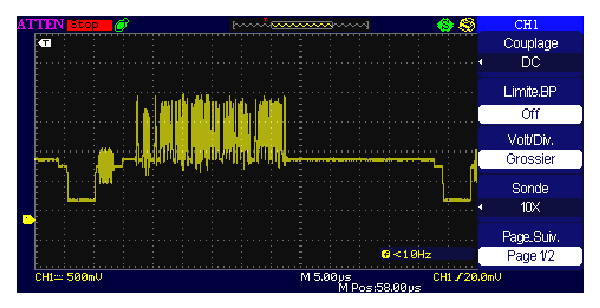
\includegraphics{images/1ligne.eps}}
\psframe[linewidth=0.05,linecolor=blue,dimen=outer](1.86,0.28359374)(0.2,-1.3364062)
\psframe[linewidth=0.05,linecolor=blue,dimen=outer](7.76,0.22359376)(6.78,-1.2964063)
\psframe[linewidth=0.05,linecolor=red,dimen=outer](6.72,0.76359373)(1.92,-1.3564062)
\usefont{T1}{ppl}{m}{n}
\rput(5.0892186,-3.0264063){Synchronisation de ligne}
\usefont{T1}{ppl}{m}{n}
\rput(5.1634374,3.0335937){Luminance pour une ligne}
\psline[linewidth=0.05cm,linecolor=red,arrowsize=0.153cm 2.0,arrowlength=1.4,arrowinset=0.4]{->}(3.64,2.8235939)(3.7,0.7835938)
\psline[linewidth=0.05cm,linecolor=blue,arrowsize=0.173cm 2.0,arrowlength=1.4,arrowinset=0.4]{->}(2.84,-2.8764062)(1.76,-1.3364062)
\psline[linewidth=0.05cm,linecolor=blue,arrowsize=0.153cm 2.0,arrowlength=1.4,arrowinset=0.4]{->}(6.8,-2.7964063)(7.02,-1.2964063)
\end{pspicture} 
}
\scalebox{1} % Change this value to rescale the drawing.
{
\begin{pspicture}(0,-2.34)(9.6,2.34)
\rput(4.8,0.0){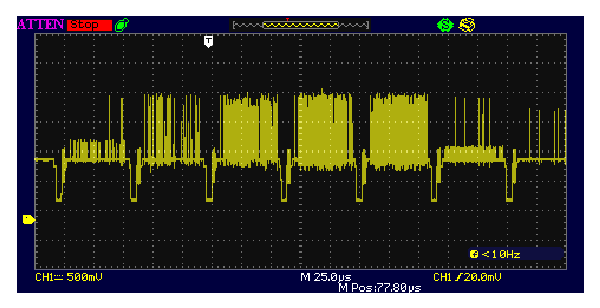
\includegraphics{images/quelquelignes.eps}}
\end{pspicture} 
}

\end{center}


Il y a ensuite la synchronisation de frame qui est véhiculée par un signal numérique (il y passe aussi par cet endroit des informations sur la sources du signal, ici aucun car c'est une simple caméra).

\begin{center}

\scalebox{1} % Change this value to rescale the drawing.
{
\begin{pspicture}(0,-2.34)(9.6,2.34)
\rput(4.8,0.0){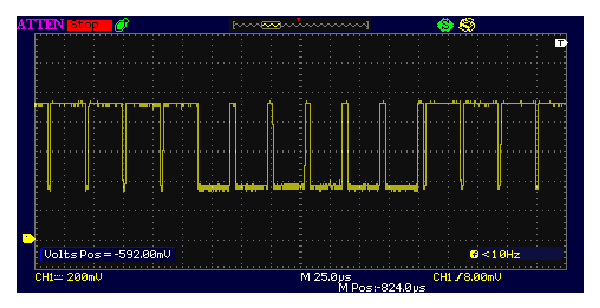
\includegraphics{images/sincronisation.eps}}
\end{pspicture} 
}
\end{center}

Ce qui donne une image sous cette forme :

\begin{center}
\centering
\scalebox{1} % Change this value to rescale the drawing.
{
\begin{pspicture}(0,-2.34)(9.6,2.34)
\rput(4.8,0.0){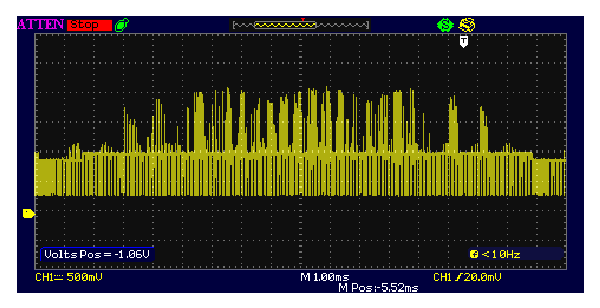
\includegraphics{images/625lignes.eps}}
\end{pspicture} 
}

\end{center}

\subsection{Émetteur UHF}

\begin{center}
\scalebox{0.5} % Change this value to rescale the drawing.
{
\begin{pspicture}(0,-7.03)(24.62,7.03)
\rput(12.31,0.0){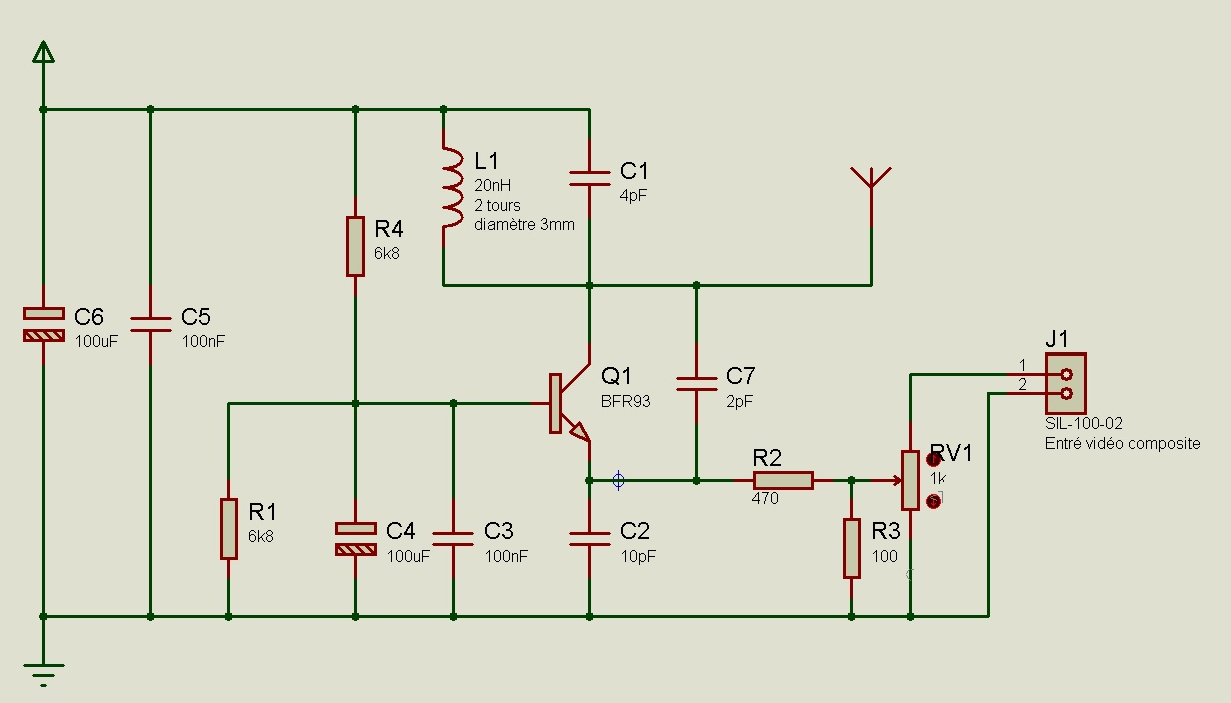
\includegraphics{/media/klafyvel/HEL2014/PI/dossier/images/emetteur.eps}}
\end{pspicture} 
}
\end{center}

L'émetteur est basé sur un oscillateur Colpitts, ce qui nous permet d'obtenir une fréquence élevée et stable avec seulement un transistor et quelques composants.
La fréquence de ce type d’oscillateur est donné par :

\[
f = \frac{1}{2\pi \sqrt{L_1 \times \frac{C_7 \times C_2}{C_7+C_2}}}
\]

J'ai donc réglé la fréquence de l'émetteur pour être entre la chaîne 58 et 60, soit entre  759,25 MHz
 et 783,25 MHz, qui donne $C_7 = 2pF$, $C_2 = 10pF$ et $L_1 = 20nH$. Donc
\[
f = \frac{1}{ 2 \pi \sqrt{ 2.10^{-8} \frac{2 \cdot 10^{-12} \times 1 \cdot 10^{-11}}{2 \cdot 10^{-12} + 1 \cdot 10^{-11}}}} = 8.71728 \cdot 10^8 Hz
\]
Soit 871,728 MHz.


La transmission de données se fait par modulation de la fréquence, donc pour faire passer  les informations vidéo il suffit de faire varier la tension aux bornes du condensateur, ce qui se répercute sur la fréquence d’oscillation. L'amplitude de modulation de la fréquence doit pouvoir être réglable pour avoir une transmission optimale.
Donc le signal vidéo composite passe par un potentiomètre, nous permettant ainsi de modifier son amplitude, puis le pont de résistance ne fait que protéger la caméra en cas de retour de tension de l'oscillateur.


L’antenne est directement mise sur la sortie de l'oscillateur, sa longueur dépend de la longueur d'onde, qui se calcule par la relation $\lambda \frac{c}{f}$.
c vaut la vitesse de l'électricité soit 299 792 548 $m.s^{-1}$. Soit $\lambda = \frac{299 792 458}{871,728 \cdot 10^6} = 0,3439 m $


Aux vues de la puissance de transmission et du peu de place libre , j'ai choisi de prendre un multiple de la longueur d'onde, soit, en divisant par 6 57,3mm.

\section{Récepteur vidéo}

La réception se fait par un TUNER d'un ancien téléviseur portable, sur lequel la sélection de la fréquence des chaînes se fait par la variation de tension sur une entrée du TUNER, puis il y a une sortie composite directement reliée à une entrée du circuit intégré CSC5151 qui contrôle le tube cathodique. Le signal composite est récupéré pour être affiché sur un écran LCD fixé sur la manette.